\section{因果Green函数}
\label{sec:lde-green}

常数变易公式中，积分号里的$\bm{\Phi}(t,s)$单独拿出来是什么意思？做一个思想实验：系统原本静止，在时刻$s$突然敲它一下，随后观察它的响应。

\paragraph{窄脉冲的极限}
“敲一下”可以用一个窄而高的矩形输入来描述。取单位面积的脉冲：在$[s,s+\varepsilon)$上输入为$\varepsilon^{-1}\bm{e}_j$，其余时刻为零，$\bm{e}_j$是第$j$个坐标方向。以零初值代入式~\eqref{eq:lde-variation-of-constants}。输入开始前响应为零，输入结束后，当$t\geq s+\varepsilon$时，
\[
 \bm{x}_{\varepsilon}(t)=\frac{1}{\varepsilon}\int_s^{s+\varepsilon}\bm{\Phi}(t,r)\bm{e}_j\,\mathrm{d}r.
\]

由定理~\ref{thm:lde-transition-properties}的(3)，$\bm{\Phi}(t,r)$对$r$连续，所以$\varepsilon\to0$时积分平均趋于$r=s$处的值。对每个$t>s$，
\begin{equation}
 \lim_{\varepsilon\to0^+}\bm{x}_{\varepsilon}(t)=\bm{\Phi}(t,s)\bm{e}_j,
 \label{eq:lde-pulse-limit}
\end{equation}
而$t<s$时响应恒为零。$\bm{\Phi}(t,s)$的第$j$列就是这样一种响应：在时刻$s$沿第$j$个方向敲一下，系统在时刻$t$的状态。

\begin{definition}[因果Green函数]
\label{def:lde-causal-green}
对$t,s\in I$，线性系统$\dot{\bm{x}}=\bm{A}(t)\bm{x}+\bm{g}$的\term{因果Green函数}（causal Green's function）定义为
\begin{equation}
 \bm{G}(t,s)=\bm{\Phi}(t,s)\mathbb{I}_{[s,\infty)}(t),
 \label{eq:lde-causal-green}
\end{equation}
其中$\mathbb{I}_{[s,\infty)}$是区间$[s,\infty)$的示性函数。$\bm{G}(t,s)$在$t<s$时为零。
\end{definition}

有了$\bm{G}$，零状态响应（记为$\bm{x}_{\mathrm{zs}}$）可以写成对整段时间的积分。设$\bm{g}$在$[t_0,T]$上连续，$t\in[t_0,T]$，由$\bm{G}$在$s>t$时为零，得
\begin{equation}
 \bm{x}_{\mathrm{zs}}(t)=\int_{t_0}^{T}\bm{G}(t,s)\bm{g}(s)\,\mathrm{d}s.
 \label{eq:lde-green-solution}
\end{equation}
积分虽然延伸到$T$，实际只用到$s\leq t$的输入。这就是“因果”的含义：未来的输入不影响现在的状态。

$\bm{G}$在对角线$t=s$处有跳变。从$t<s$一侧的$\bm{0}$跳到$t>s$一侧的$\bm{I}$，所以
\begin{equation}
 \bm{G}(s^+,s)-\bm{G}(s^-,s)=\bm{I}.
 \label{eq:lde-green-jump}
\end{equation}
$t\neq s$时，$\bm{G}$对$t$满足齐次方程。工程和物理中常把这两条性质合写成
\[
 (\partial_t-\bm{A}(t))\bm{G}(t,s)=\delta(t-s)\bm{I}.
\]
这里的$\delta$不是普通函数，这个写法只是式~\eqref{eq:lde-pulse-limit}和跳变条件~\eqref{eq:lde-green-jump}的简写。

\paragraph{标量例子与脉冲响应}
常系数时$\bm{G}$只依赖时间差，$\bm{G}(t,s)=\bm{H}(t-s)$，其中
\begin{equation}
 \bm{H}(t)=\mathrm{e}^{t\bm{A}}\mathbb{I}_{[0,\infty)}(t).
 \label{eq:lde-constant-green}
\end{equation}
取$t_0=0$，零状态响应就是一个卷积：
\begin{equation}
 \bm{x}_{\mathrm{zs}}(t)=\int_0^t\bm{H}(t-s)\bm{g}(s)\,\mathrm{d}s.
 \label{eq:lde-convolution-response}
\end{equation}
时变系统没有这个简化。例如$\dot{x}=-2tx+g$的Green函数是
\[
 G(t,s)=\mathrm{e}^{s^2-t^2}\mathbb{I}_{[s,\infty)}(t),
\]
它依赖$s$和$t$本身，而不只是$t-s$。

高阶方程$p(\mathrm{D})x=g$由式~\eqref{eq:lde-companion}进入状态形式，输入只作用在最后一个分量上。单位脉冲让状态跳变$\bm{e}_n$：只有最高一阶导数$\mathrm{D}^{n-1}x$跳变$1$，$x$及更低阶的导数仍然连续。所以\term{脉冲响应}（impulse response）$w$是齐次方程在下列初值下的解：
\begin{equation}
 p(\mathrm{D})w=0,\qquad \mathrm{D}^{j}w(0)=0\ (j\leq n-2),\quad \mathrm{D}^{n-1}w(0)=1.
 \label{eq:lde-impulse-response}
\end{equation}
相应的零状态响应是$x(t)=\int_0^tw(t-s)g(s)\,\mathrm{d}s$。

对$\ddot{x}+3\dot{x}+2x=g$，$w$是$\mathrm{e}^{-t}$和$\mathrm{e}^{-2t}$的组合。由$w(0)=0$、$\dot{w}(0)=1$解出
\[
 w(t)=\mathrm{e}^{-t}-\mathrm{e}^{-2t},\qquad t\geq0.
\]
它就是例~\ref{ex:lde-step-response}中积分的被积函数，$g\equiv1$的响应正是$\int_0^tw(r)\,\mathrm{d}r$。图~\ref{fig:lde-pulse-limit}验证了脉冲极限：宽度$\varepsilon$减小时，矩形输入越来越高，响应却收敛到同一条曲线$w$。

\begin{BookInlineFigure}
  \centering
  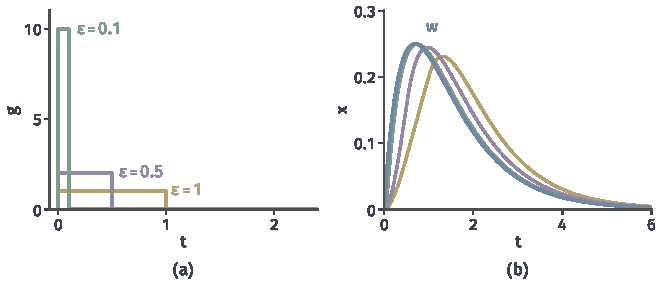
\includegraphics[width=112mm]{figures/06-differential-equations/01-ordinary-differential-equations/matplotlib/lde-pulse-limit/figure.pdf}
  \caption{窄脉冲的响应趋于脉冲响应，方程$\ddot{x}+3\dot{x}+2x=g$，零初值。(a)单位面积的矩形输入，宽度$\varepsilon=1,0.5,0.1$。(b)相同颜色的线是对应的精确响应，蓝线是脉冲响应$w=\mathrm{e}^{-t}-\mathrm{e}^{-2t}$。}
  \label{fig:lde-pulse-limit}
\end{BookInlineFigure}

\paragraph{输入是脉冲的叠加}
叠加原理让这个思想实验变成计算方法。把输入切成许多细长的矩形，每个矩形近似一次脉冲，响应是它们各自响应的总和；矩形变窄时，这个和就成为积分~\eqref{eq:lde-green-solution}。

取$\dot{x}=-x+g$，$g(t)=1+\cos t$，$x(0)=0$，此时$G(t,s)$在$t\geq s$时等于$\mathrm{e}^{-(t-s)}$。直接积分时用到
\[
 \int_0^t\mathrm{e}^{-(t-s)}\cos s\,\mathrm{d}s=\frac{\cos t+\sin t-\mathrm{e}^{-t}}{2},
\]
于是
\[
 x(t)=1+\frac{\cos t+\sin t}{2}-\frac32\mathrm{e}^{-t}.
\]

图~\ref{fig:lde-impulse-superposition}把$[0,6]$切成宽$0.5$的矩形。(b)中每条黄线是一个矩形的响应：输入期间上升，输入结束后按$\mathrm{e}^{-t}$衰减。它们的和（绿线）已经很接近精确解（蓝线），矩形取得更窄时差别还会减小。

\begin{BookInlineFigure}
  \centering
  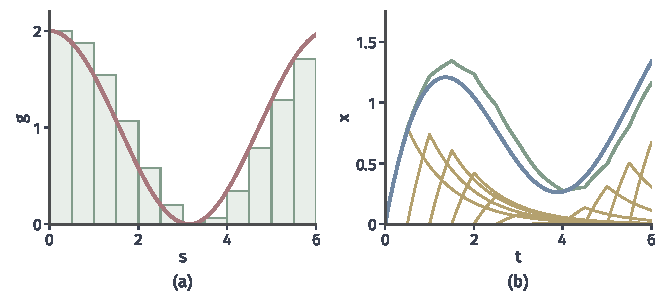
\includegraphics[width=112mm]{figures/06-differential-equations/01-ordinary-differential-equations/matplotlib/lde-impulse-superposition/figure.pdf}
  \caption{输入响应是脉冲响应的叠加，方程$\dot{x}=-x+g$，$x(0)=0$。(a)红线是输入$g=1+\cos s$，绿色矩形是宽$0.5$的分段常值近似，高度取矩形左端的$g$值。(b)黄线是单个矩形输入的响应，绿线是它们的和，蓝线是精确解。}
  \label{fig:lde-impulse-superposition}
\end{BookInlineFigure}

\paragraph{把算子看成下三角矩阵}
把函数看成无限维向量，可以换一个角度理解$\bm{G}$。在等距网格$t_k=t_0+kh$上，式~\eqref{eq:lde-green-solution}近似为一个矩阵乘向量：
\[
 x(t_i)\approx\sum_{j<i}hG(t_i,t_j)g(t_j).
\]
矩阵的第$(i,j)$元是$hG(t_i,t_j)$。第$j$列是在时刻$t_j$敲一下之后的响应序列，第$i$行说明时刻$t_i$的状态怎样加权历史上的输入。

$G(t_i,t_j)$在$j>i$时为零，这个矩阵是下三角的，所以因果性就是下三角结构。图~\ref{fig:lde-green-heatmap}(a)画出$\dot{x}=-x+g$的$G(t,s)$，只有对角线上方有值。类比的限度在于对角线：矩阵元是有限数，而$G$在对角线上的跳变对应着连续问题中$\delta$的位置，它不是任何矩阵元能单独表示的。

同样叫Green函数，边值问题的情形却不同。图~\ref{fig:lde-green-heatmap}(b)是$-\mathrm{d}^2u/\mathrm{d}x^2=f$、$u(0)=u(1)=0$的积分核$\min(x,s)(1-\max(x,s))$，它在对角线两侧都不为零。空间中的边界条件同时从两端约束解，一点的源影响所有位置，没有“先后”可言。这种边值Green函数由第~\ref{chap:elliptic-equations}章介绍。

\begin{BookInlineFigure}
  \centering
  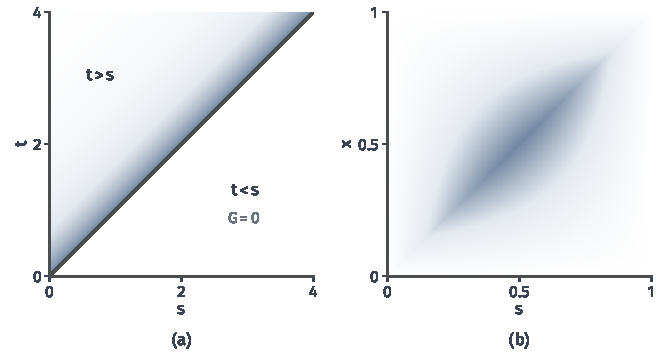
\includegraphics[width=112mm]{figures/06-differential-equations/01-ordinary-differential-equations/matplotlib/lde-green-heatmap/figure.pdf}
  \caption{因果Green函数与边值积分核的对比，颜色越深表示数值越大。(a)$G(t,s)=\mathrm{e}^{-(t-s)}\mathbb{I}_{[s,\infty)}(t)$，深灰线是对角线$t=s$，其下方$G$为零，体现因果性。(b)两点边值问题的核$\min(x,s)(1-\max(x,s))$，对角线两侧都不为零。}
  \label{fig:lde-green-heatmap}
\end{BookInlineFigure}
